% Options for packages loaded elsewhere
\PassOptionsToPackage{unicode}{hyperref}
\PassOptionsToPackage{hyphens}{url}
\documentclass[
]{article}
\usepackage{xcolor}
\definecolor{urblue}{RGB}{0,84,159}
\usepackage{amsmath,amssymb}
\setcounter{secnumdepth}{-\maxdimen} % remove section numbering
\usepackage{iftex}
\ifPDFTeX
  \usepackage[T1]{fontenc}
  \usepackage[utf8]{inputenc}
  \usepackage{textcomp} % provide euro and other symbols
\else % if luatex or xetex
  \usepackage{unicode-math} % this also loads fontspec
  \defaultfontfeatures{Scale=MatchLowercase}
  \defaultfontfeatures[\rmfamily]{Ligatures=TeX,Scale=1}
\fi
\usepackage{lmodern}
\ifPDFTeX\else
  % xetex/luatex font selection
\fi
% Use upquote if available, for straight quotes in verbatim environments
\IfFileExists{upquote.sty}{\usepackage{upquote}}{}
\IfFileExists{microtype.sty}{% use microtype if available
  \usepackage[]{microtype}
  \UseMicrotypeSet[protrusion]{basicmath} % disable protrusion for tt fonts
}{}
\makeatletter
\@ifundefined{KOMAClassName}{% if non-KOMA class
  \IfFileExists{parskip.sty}{%
    \usepackage{parskip}
  }{% else
    \setlength{\parindent}{0pt}
    \setlength{\parskip}{6pt plus 2pt minus 1pt}}
}{% if KOMA class
  \KOMAoptions{parskip=half}}
\makeatother
\usepackage{longtable,booktabs,array}
\newcounter{none} % for unnumbered tables
\usepackage{calc} % for calculating minipage widths
% Correct order of tables after \paragraph or \subparagraph
\usepackage{etoolbox}
\makeatletter
\patchcmd\longtable{\par}{\if@noskipsec\mbox{}\fi\par}{}{}
\makeatother
% Allow footnotes in longtable head/foot
\IfFileExists{footnotehyper.sty}{\usepackage{footnotehyper}}{\usepackage{footnote}}
\makesavenoteenv{longtable}
\usepackage{graphicx}
\usepackage{subcaption}
\usepackage{float} % <-- ADDED: Fixes the "Unknown float option H" error
% Make figure captions bold (label + text)
\captionsetup[figure]{labelfont=bf,textfont=bf}
% Force graphics to be included even if something enables draft mode
\setkeys{Gin}{draft=false}
\makeatletter
\newsavebox\pandoc@box
\newcommand*\pandocbounded[1]{% scales image to fit in text height/width
  \sbox\pandoc@box{#1}%
  \Gscale@div\@tempa{\textheight}{\dimexpr\ht\pandoc@box+\dp\pandoc@box\relax}%
  \Gscale@div\@tempb{\linewidth}{\wd\pandoc@box}%
  \ifdim\@tempb\p@<\@tempa\p@\let\@tempa\@tempb\fi% select the smaller of both
  \ifdim\@tempa\p@<\p@\scalebox{\@tempa}{\usebox\pandoc@box}%
  \else\usebox{\pandoc@box}%
  \fi%
}
% Set default figure placement to htbp
\def\fps@figure{htbp}
\makeatother
\setlength{\emergencystretch}{3em} % prevent overfull lines
\providecommand{\tightlist}{%
  \setlength{\itemsep}{0pt}\setlength{\parskip}{0pt}}
\usepackage{bookmark}
\IfFileExists{xurl.sty}{\usepackage{xurl}}{} % add URL line breaks if available
\urlstyle{same}
\hypersetup{
  hidelinks,
  pdfcreator={LaTeX via pandoc}}
  
% --- IEEE BIBLIOGRAPHY CONFIGURATION ---
\usepackage[style=ieee, backend=biber]{biblatex}
\addbibresource{references.bib}

\title{QoS-Aware Resource Allocation and Performance Evaluation for 5G Network Slicing Under Nakagami-$m$ Fading: A Multi-RB Uplink H-NOMA Study for eMBB and URLLC}
\author{Author Name}
\date{\today}

\begin{document}

% Front matter (roman)
\pagenumbering{roman}

% Cover page
\begin{titlepage}
\centering

%==================== HEADER ====================%
\noindent
\begin{minipage}[t]{0.48\textwidth}
    \vspace{0pt}
    
\includegraphics[width=4.5cm]{media/ur_logo.jpg}
\end{minipage}
\hfill
\begin{minipage}[t]{0.48\textwidth}
    \vspace{12pt}
    \raggedleft
    \color{urblue}\textbf{COLLEGE OF SCIENCE}\\
    \color{urblue}\textbf{AND TECHNOLOGY}
\end{minipage}
\vspace{2cm}

%==================== SCHOOL ====================%
{\Large\bfseries\color{urblue} SCHOOL OF ENGINEERING} \\
\vspace{0.7cm}
{\large\bfseries DEPARTMENT OF ELECTRICAL AND ELECTRONICS}
\vspace{0.3cm}
{\large\bfseries ENGINEERING}
\vspace{1cm}

%==================== PROJECT TITLE ====================%
{\large\bfseries
QoS-Aware Resource Allocation and Performance\\
Evaluation for 5G Network Slicing Under\\
Nakagami-$m$ Fading: A Multi-RB Uplink\\
H-NOMA Study for eMBB and URLLC
}

\vspace{1cm}

%==================== STUDENTS ====================%
\textit{
Nahum IGIRANEZA -- 222018327\\[0.15cm]
Louis Clement ABAYO -- 222004020\\[0.15cm]
Shema Dolph NSENGIYUMVA -- 222009353
}

\vspace{0.8cm}

June 2026

\vspace{1.2cm}

{\large\bfseries Undergraduate Final Year Project}

\vfill

%==================== DEGREE BOX ====================%
\fcolorbox{black}{cyan!55}{
\begin{minipage}{0.94\textwidth}
\centering
\vspace{0.15cm}

\textbf{Bachelor of Science in Electronics and Telecommunication Engineering}

\vspace{0.15cm}

\textbf{Supervisor: Prof. Charles KABIRI}

\vspace{0.15cm}
\end{minipage}
}

\vspace{0.6cm}

\begin{flushleft}
\textbf{Project ID:} EEE/ETE/2025-2026/01
\end{flushleft}
\end{titlepage}

% Dedication
\section*{Dedication}
\addcontentsline{toc}{section}{Dedication}
\vspace{1cm}

We would like to dedicate this work to:

\begin{itemize}
    \item Almighty God, for whom our hearts are full of gratitude.
    
    \item Our families, for their continuous support and motivation throughout our journey.
    
    \item Our lecturers and academic supervisor, for their guidance, support, and valuable insights.
    
    \item Our classmates and friends, for their encouragement and companionship during our studies.
\end{itemize}

\vspace*{\fill}
\clearpage

% Approval and Certification
\section*{Approval and Certification}
\addcontentsline{toc}{section}{Approval and Certification}

I hereby declare that this final year project report titled
\textit{``QoS-Aware Resource Allocation and Performance
Evaluation for 5G Network Slicing Under
Nakagami-m Fading: A Multi-RB Uplink
H-NOMA Study for eMBB and URLLC''}
is our own original work and has not been submitted, either in whole or in part, for a degree or diploma at this university or any other institution. All sources of information and ideas used have been rightly acknowledged through references.

\vspace{01cm}

\noindent\begin{tabular}{@{}p{0.44\textwidth}p{0.28\textwidth}p{0.20\textwidth}@{}}
\textbf{Name} & \textbf{Student ID} & \textbf{Signature}\\[0.6cm]

Nahum IGIRANEZA & 222018327 & \hrulefill \\[0.7cm]

Louis Clement ABAYO & 222004020 & \hrulefill \\[0.7cm]

Shema Dolph NSENGIYUMVA & 222009353 & \hrulefill \\


\end{tabular}

\vspace{1cm}

\textbf{Supervisor's Approval}

\vspace{0.3cm}

Name: Prof. Charles KABIRI

\vspace{0.3cm}

Signature: \hrulefill
\clearpage

% Acknowledgement
\section*{Acknowledgement}
\addcontentsline{toc}{section}{Acknowledgement}

First and foremost, we would like to express our sincere gratitude to the Almighty God for the strength, wisdom, and perseverance granted throughout this academic journey.

We are deeply indebted to our supervisor, Prof. Charles KABIRI, for the invaluable guidance, constructive criticism, and unwavering support throughout this project. Your expertise and patience have been instrumental in shaping the quality of this work.

We extend our heartfelt thanks to the faculty and staff of the Department of Electrical and Electronics Engineering at the University of Rwanda.

Finally, we are eternally grateful to our families and friends for their moral support, encouragement, and understanding during the demanding periods of this research.
\clearpage

% Abstract
\section*{Abstract}
\addcontentsline{toc}{section}{Abstract}

This project investigates QoS-aware resource allocation for 5G network slicing between eMBB and URLLC services under Nakagami-m fading conditions.

The study addresses the challenge of allowing high-throughput broadband traffic and ultra-reliable low-latency traffic to share limited uplink radio resources.

A multi-resource-block H-NOMA system model is developed, where power-domain sharing and successive interference cancellation are used to separate the two service slices.

The power allocation factor α is used to control the trade-off between eMBB capacity improvement and URLLC reliability protection.

Analytical expressions for outage probability, SINR, capacity, and effective throughput are derived and evaluated through MATLAB-based simulation.

The results show that allocating more power to eMBB improves throughput but can reduce URLLC reliability due to lower URLLC power and stronger interference.

Therefore, the project demonstrates that reliable 5G slicing requires QoS-constrained allocation rather than simple throughput maximization.
\clearpage

% Table of contents / figures / tables
\tableofcontents
\clearpage

\listoffigures
\addcontentsline{toc}{section}{List of Figures}
\clearpage

\listoftables
\addcontentsline{toc}{section}{List of Tables}
\clearpage

% List of abbreviations, acronyms and symbols
\section*{List of Abbreviations and Acronyms}
\addcontentsline{toc}{section}{List of Abbreviations and Acronyms}
\begin{tabular}{p{0.25\textwidth} p{0.7\textwidth}}
5G & Fifth Generation \\
QoS & Quality of Service \\
eMBB & Enhanced Mobile Broadband \\
URLLC & Ultra-Reliable Low-Latency Communication \\
mMTC & Massive Machine-Type Communications \\
H-NOMA & Heterogeneous Non-Orthogonal Multiple Access \\
NOMA & Non-Orthogonal Multiple Access \\
OMA & Orthogonal Multiple Access \\
H-OMA & Heterogeneous Orthogonal Multiple Access \\
SINR & Signal-to-Interference-plus-Noise Ratio \\
SNR & Signal-to-Noise Ratio \\
SIC & Successive Interference Cancellation \\
RB & Resource Block \\
gNodeB (gNB) & Next Generation Node B (5G Base Station) \\
PSD & Power Spectral Density \\
CDF & Cumulative Distribution Function \\
PDF & Probability Density Function \\
GHz & Gigahertz \\
MHz & Megahertz \\
kHz & Kilohertz \\
Hz & Hertz \\
dB & Decibel \\
dBm & Decibel-milliwatts \\
MATLAB & MATrix LABoratory \\
MC & Monte Carlo \\
3GPP & 3rd Generation Partnership Project \\
TS & Technical Specification \\
NR & New Radio \\
NG-RAN & Next Generation Radio Access Network \\
NRM & Network Resource Model \\
IS & Information Service \\
VTC & Vehicular Technology Conference \\
IEEE & Institute of Electrical and Electronics Engineers \\
\end{tabular}
\clearpage

\section*{List of Symbols}
\addcontentsline{toc}{section}{List of Symbols}

\begin{tabular}{p{0.25\textwidth} p{0.7\textwidth}}
$\alpha$ & Power Allocation Factor \\
$\gamma$ & SINR/SNR Variable \\
$\gamma_{th}$ & SINR Threshold \\
$P_t$ & Total Transmit Power \\
$P_B$ & eMBB Transmit Power \\
$P_U$ & URLLC Transmit Power \\
$N_B$ & eMBB Noise Power \\
$N_U$ & URLLC Noise Power \\
$C_B$ & eMBB Capacity \\
$C_U$ & URLLC Capacity \\
$T_B$ & eMBB Effective Throughput \\
$T_U$ & URLLC Effective Throughput \\
$P_{out}$ & Outage Probability \\
$NF$ & Noise Figure \\
$PL$ & Path Loss \\
$f_c$ & Carrier Frequency \\
$W_{RB}$ & Resource Block Bandwidth \\
$N_{RB}$ & Number of Resource Blocks \\
\end{tabular}
\clearpage

% --------------------
% Main matter (arabic)
% --------------------
\pagenumbering{arabic}

\section{Chapter 1: Introduction}\label{chapter-1-introduction}

\subsection{1.1 Background}\label{background}

Fifth-generation (5G) wireless systems are designed to support heterogeneous service classes over a common network infrastructure. Enhanced Mobile Broadband (eMBB) services require high data rates and efficient spectrum utilization, while Ultra-Reliable Low-Latency Communication (URLLC) services demand stringent reliability and latency guarantees. Supporting these diverse requirements simultaneously presents significant challenges for radio resource management and network slicing \parencite{Popovski2018}.

This project develops a QoS-aware resource allocation and performance evaluation framework for 5G network slicing under Nakagami-m fading conditions. The framework considers the allocation of radio resources among heterogeneous service slices while accounting for differences in bandwidth requirements, transmission reliability, and quality-of-service constraints. Heterogeneous Non-Orthogonal Multiple Access (H-NOMA) is adopted as the resource-sharing mechanism, enabling the investigation of outage probability, signal-to-interference-plus-noise ratio (SINR), capacity, effective throughput, and QoS feasibility under various resource allocation strategies \parencite{Tominaga2021}.

\subsection{1.2 Problem Statement}\label{problem-statement}

The central problem is to determine how a fixed uplink transmit power
budget should be split between eMBB and URLLC so that eMBB receives
enough capacity while URLLC remains reliable. The challenge arises
because increasing the eMBB power fraction improves eMBB SNR and
capacity, but it reduces URLLC transmit power and increases the
interference seen by URLLC during the first SIC decoding stage.
Therefore, the power allocation factor alpha must be selected using QoS
constraints rather than only by maximizing total throughput \parencite{Feng2021}.

\subsection{1.3 Research Objectives}\label{research-objectives}

\begin{enumerate}
\def\labelenumi{\arabic{enumi}.}
\item 
To develop a multi-resource-block uplink network slicing model for eMBB and URLLC services incorporating realistic 5G bandwidth allocation using usable resource blocks and wireless propagation characterized by distance-dependent path loss and Nakagami-m fading channels.
\item
To formulate a QoS-aware power allocation mechanism based on the power allocation factor \(α\) for resource sharing between service slices.
\item
  To derive analytical outage probability expressions for eMBB and URLLC services under integer Nakagami-m fading and evaluate system performance using outage probability, SINR, achievable capacity, effective throughput, and QoS feasibility metrics.
\item
 To identify feasible resource allocation regions and determine the resource allocation factor that maximizes overall system throughput while simultaneously satisfying the QoS requirements of both eMBB and URLLC services. 

\end{enumerate}

\subsection{1.4 Scope and Limitations}\label{scope-and-limitations}

The scope is restricted to one eMBB user and one URLLC user transmitting
to one gNodeB. The MATLAB implementation considers alpha-sweep analysis
at a fixed total transmit power of 30 dBm, Nakagami-m parameters
m in \{1,2,3,4\}, and Monte Carlo validation using 2 x 10\^{}5 channel
samples for outage and capacity-related plots.

\clearpage

\section{Chapter 2: Literature
Review}\label{chapter-2-literature-review}

\subsection{2.1 5G Network Slicing}\label{g-network-slicing}

Network slicing allows one physical 5G network to be partitioned into
logical slices with different QoS requirements. In the radio access
network, slicing decisions include bandwidth allocation, scheduling, and
interference management. The eMBB slice is generally
throughput-oriented, while the URLLC slice is reliability-oriented. This
difference creates a trade-off because both services may require access
to limited radio resources \parencite{Zhang2017}.

\subsection{2.2 QoS-Aware Resource Allocation in 5G
Networks}\label{qos-aware-resource-allocation-in-5g-networks}

Resource allocation is one of the fundamental challenges in 5G systems
because multiple services with heterogeneous QoS requirements must share
limited radio resources. QoS-aware resource allocation refers to the
process of allocating bandwidth, transmit power, and scheduling
opportunities while ensuring that predefined service requirements are
satisfied.

For eMBB services, resource allocation algorithms typically prioritize
throughput and spectral efficiency. In contrast, URLLC services require
stringent reliability and latency guarantees. Several studies have shown
that maximizing overall throughput alone may result in unacceptable
reliability degradation for URLLC users. Therefore, modern resource
allocation frameworks employ QoS constraints to balance the conflicting
requirements of different service classes \parencite{Zhang2017}.

In network slicing environments, power allocation is widely used as a
practical mechanism for controlling service performance because it
directly influences SINR, outage probability, and achievable data rates.

\subsection{2.3 Heterogeneous NOMA for eMBB and
URLLC}\label{heterogeneous-noma-for-embb-and-urllc}

Heterogeneous NOMA (H-NOMA) extends the NOMA principle to users or
slices with different QoS requirements. In this project, the base
station applies SIC by decoding the URLLC signal first while treating
eMBB as interference. After URLLC is decoded and cancelled, eMBB is
decoded using a post-SIC SNR \parencite{Popovski2018}. This ordering is consistent with the
reliability diversity concept, because URLLC must be protected despite
sharing resources with a high-rate eMBB transmission .


\subsection{2.4 Performance Evaluation Metrics for Network
Slicing}\label{performance-evaluation-metrics-for-network-slicing}

The effectiveness of resource allocation strategies is commonly
evaluated using performance metrics such as outage probability,
signal-to-interference-plus-noise ratio (SINR), achievable capacity,
effective throughput, latency, and reliability.

Outage probability is particularly important for URLLC because it
measures the likelihood that a communication link fails to satisfy its
required SINR threshold. Capacity and throughput metrics are more
relevant to eMBB services because they quantify achievable data rates
and spectrum utilization efficiency \parencite{Men2017}.

These performance indicators provide a quantitative basis for evaluating
whether resource allocation decisions satisfy the QoS requirements of
different service slices.

\clearpage

\section{Chapter 3: System Model and
Architecture}\label{chapter-3-system-model-and-architecture}

This chapter presents the proposed QoS-aware uplink H-NOMA system for 5G
network slicing. The system consists of one enhanced Mobile Broadband
(eMBB) user, one Ultra-Reliable Low-Latency Communication (URLLC) user,
and one 5G base station or gNodeB. The eMBB user represents a
high-throughput service, while the URLLC user represents a low-latency
and high-reliability service. The main purpose of the model is to
determine how the total uplink transmit power should be split between
the two slices so that both service requirements can be satisfied.

\subsection{3.1 System Architecture}\label{system-architecture}

In the proposed architecture, the eMBB and URLLC users transmit
simultaneously to the same gNodeB. The gNodeB applies successive
interference cancellation (SIC) to separate the two signals. Since URLLC
has stricter reliability requirements, the receiver first decodes the
URLLC signal while treating the eMBB signal as interference. After the
URLLC signal is decoded, it is cancelled from the received signal. The
eMBB signal is then decoded after SIC \parencite{Popovski2018}.

The power allocation factor \(α\) controls the power split between the two
slices. The eMBB user receives \(\alpha P_{t}\), while the URLLC user
receives \((1 - \alpha)P_{t}\). Therefore, increasing \(α\) improves the
eMBB link because more power is assigned to eMBB, but it can degrade the
URLLC link because less power remains for URLLC and the eMBB
interference becomes stronger during the first SIC decoding stage. The
design problem is therefore a QoS-constrained trade-off rather than a
simple throughput maximization problem \parencite{Tominaga2021}.

\begin{figure}[htbp]
\centering
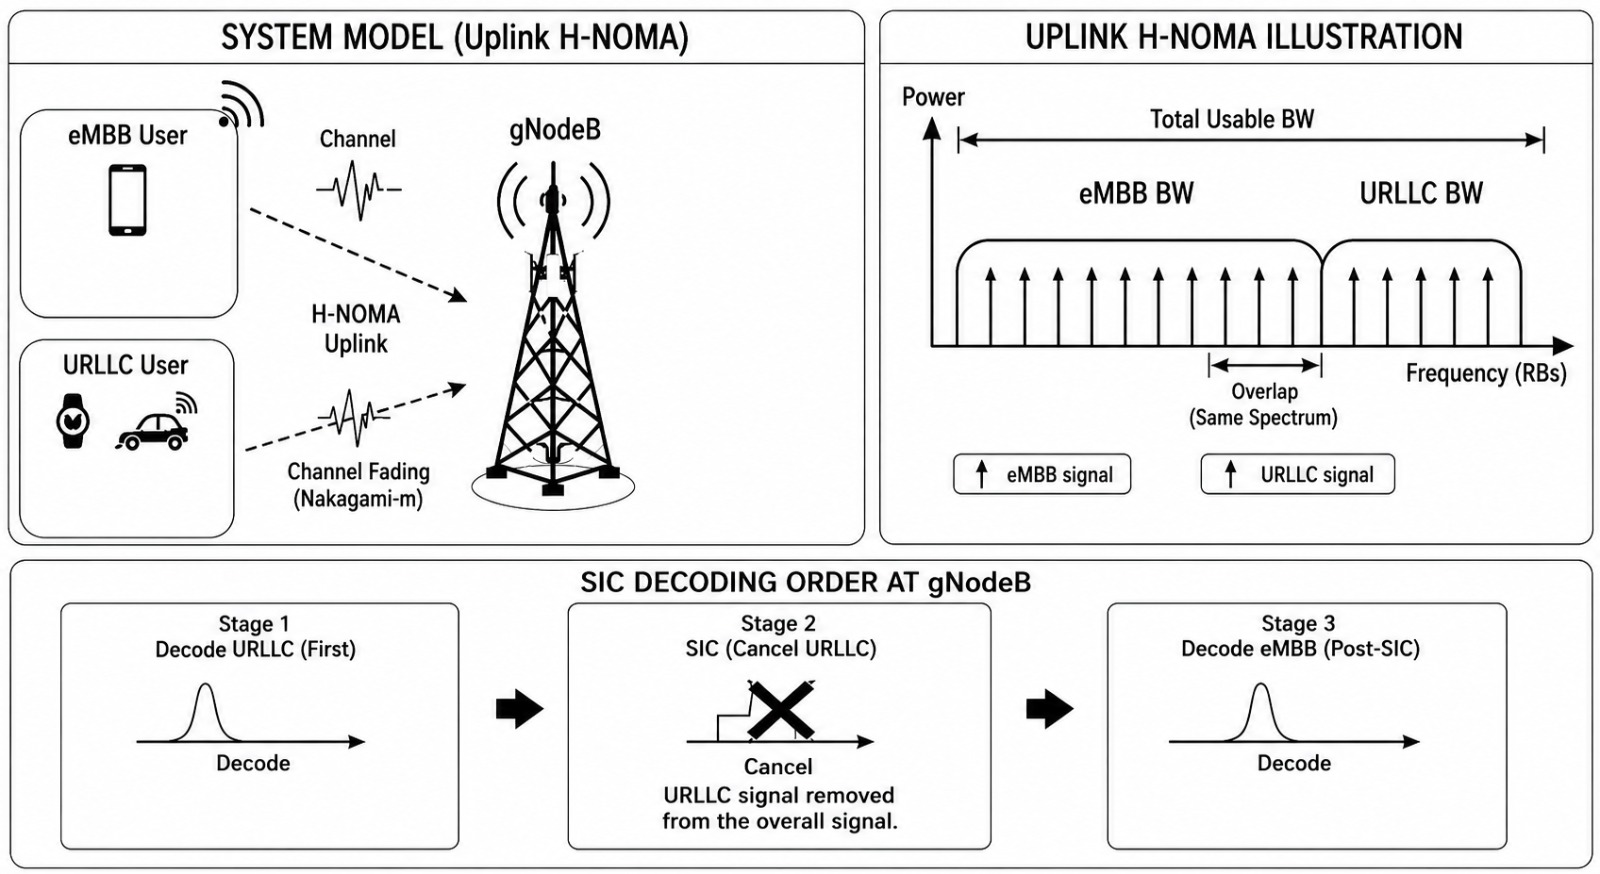
\includegraphics[width=1.0\textwidth,keepaspectratio]{media/system modal.jpeg}
\caption{\emph{Proposed uplink H-NOMA system architecture for QoS-aware 5G network slicing between eMBB and URLLC user under Nakagami-m fading.}}
\end{figure}

{\def\LTcaptype{none} % do not increment counter
\begin{longtable}[]{@{}
  >{\raggedright\arraybackslash}p{(\linewidth - 0\tabcolsep) * \real{0.9857}}@{}}
\toprule\noalign{}
\begin{minipage}[b]{\linewidth}\raggedright
\textbf{Important modelling clarification:} The RB allocation in this
work is used to define the practical bandwidth available to each service
slice for noise-power, threshold, and capacity calculations. The H-NOMA
operation is modelled through power-domain superposition and SIC at the
receiver. Therefore, the eMBB signal appears as interference during the
URLLC decoding stage, while the eMBB signal is decoded after successful
URLLC cancellation \parencite{Zhang2017}.
\end{minipage} \\
\endhead
\bottomrule\noalign{}
\end{longtable}
}

\subsection{3.2 Multi-RB Bandwidth
Model}\label{multi-rb-bandwidth-model}

A practical 5G radio channel is not represented by a single resource block. Instead, the proposed model considers a realistic 5G channel with a nominal channel bandwidth and a usable bandwidth composed of multiple resource blocks. The available resource blocks are partitioned between the eMBB and URLLC network slices, with the eMBB slice receiving a larger share of the available bandwidth and the URLLC slice receiving the remaining portion.

The bandwidth allocated to each slice is used throughout the system model and directly influences key performance parameters, including noise power, SINR requirements, and achievable capacity. Consequently, employing a multi-resource-block framework provides a more realistic representation of practical 5G network operation and enables a more accurate performance evaluation than a simplified single-resource-block model \parencite{Popovski2018}.

\subsection{3.3 Power Allocation}\label{power-allocation}

The total uplink transmit power is fixed at \(P_{t}\). The power
allocation factor \(α\) is used to divide this power between the eMBB and
URLLC users. The eMBB power increases with \(α\), while the URLLC power
decreases with \(α\).

\begin{equation}
\begin{cases}
  P_{B} = \alpha P_{t} \\
  P_{U} = (1 - \alpha)P_{t}
\end{cases}
\quad \text{for } 0 < \alpha < 1
\end{equation}

For the baseline alpha-sweep simulation,
\(P_{t}\) is power budget where RB is limited. The optimization problem searches
for the \(α\) value that maximizes the total effective throughput while
satisfying the outage and capacity constraints of both slices \parencite{Zhang2017}.

\subsection{3.4 Noise Model with Receiver Noise
Figure}\label{noise-model-with-receiver-noise-figure}

The thermal noise power is calculated from the thermal noise power
spectral density, the allocated bandwidth, and the receiver noise
figure. This is important because the eMBB slice has four times more
bandwidth than the URLLC slice; therefore, it also has four times more
thermal noise power \parencite{Men2017}.

\begin{align}
N_{B} &= N_{o} B_{B} F \\[1ex]
N_{U} &= N_{o} B_{U} F
\end{align}

\subsection{3.5 Path Loss and Average Channel Power
Gain}\label{path-loss-and-average-channel-power-gain}

The large-scale channel gain is obtained from a 3.5 GHz
distance-dependent path loss model. The model uses a reference loss term
and a path loss exponent suitable for a dense urban environment. Antenna
gains and shadowing are not included, which keeps the analysis focused
on the power allocation, fading, and interference effects .

\begin{align}
PL_{0}\text{ (dB)} &= 32.4 + 20\log(f_{c}), \quad \text{for } f_{c} \text{ in GHz} \\[1ex]
PL_{i}\text{ (dB)} &= PL_{0}\text{ (dB)} + 10n_{PL}\log(d_{i}), \quad \text{for } i \in \{B,U\} \\[1ex]
\Omega_{i} &= 10^{\frac{PL_{i}\text{ (dB)}}{10}}
\end{align}

Under the considered system parameters, the resulting average channel gains show that the URLLC user, being closer to the base station, experiences a stronger channel than the eMBB user. This difference in channel conditions plays an important role in the allocation of resources and the resulting system performance, particularly in terms of SINR and achievable capacity.

\subsection{3.6 Nakagami-m Channel
Model}\label{nakagami-m-channel-model}

Small-scale fading is modelled using the Nakagami-m distribution. This
model is flexible because m = 1 corresponds to Rayleigh fading, while
larger m values represent less severe fading conditions. The channel
power gain \(X_{i}\  = \ {|h_{i}|}^{2}\) follows a Gamma distribution
with shape parameter m and scale parameter \(\frac{\Omega_{i}}{m}\).

\begin{align}
X_{i} &= |h_{i}|^{2} \sim \text {Gamma}\left( m,\, \frac{\Omega_{i}}{m} \right), \quad \text{for } i \in \{B,U\} \\[1ex]
f_{X_{i}}(x) &= \left( \frac{m^{m}}{\Gamma(m)\Omega_{i}^{m}} \right) x^{m - 1} \exp\left( -\frac{mx}{\Omega_{i}} \right), \quad \text{for } x \geq 0 \\[1ex]
F_{X_{i}}(x) &= 1 - \exp\left( -\frac{mx}{\Omega_{i}} \right) \sum_{k = 0}^{m - 1} \frac{1}{k!} \left( \frac{mx}{\Omega_{i}} \right)^{k}
\end{align}

The finite-sum CDF in (9) is used in the analytical outage
derivations. It is valid for integer values of m, which matches the
implemented simulation values m \(∈\) \{1,2,3,4\}.

\subsection{3.7 Received Signal and SIC
Order}\label{received-signal-and-sic-order}

The received uplink signal at the gNodeB is the superposition of the
eMBB signal, the URLLC signal, and receiver noise. The gNodeB decodes
URLLC first because URLLC is the reliability-sensitive service. During
this stage, eMBB is treated as interference. After URLLC is successfully
decoded and cancelled, eMBB is decoded from the remaining signal \parencite{Tominaga2021}.

\begin{align}
y &= \sqrt{P_{B}} h_{B} X_{B} + \sqrt{P_{U}} h_{U} X_{U} + n \\[1ex]
\gamma_{U} &= \frac{P_{U} X_{U}}{P_{B} X_{B} + N_{U}} \\[1ex]
\gamma_{B} &= \frac{P_{B} X_{B}}{N_{B}}
\end{align}

In (11) shows the key H-NOMA trade-off: URLLC reliability is
affected by both its allocated power and the interference created by the
eMBB signal. In (12) is the post-SIC eMBB SNR after the URLLC
signal has been removed.

\clearpage

\section{Chapter 4: Analytical Framework and Formula
Derivations}\label{chapter-4-analytical-framework-and-formula-derivations}

This chapter derives the SINR thresholds, outage probabilities,
effective throughput, and QoS-constrained alpha-selection rule used in
the simulation. The derivations are written in a direct form so that
they can be followed and implemented in MATLAB.

\subsection{4.1 SINR Threshold
Derivation}\label{sinr-threshold-derivation}

The Shannon capacity approximation relates the achievable rate to the
SINR and the allocated bandwidth. For a slice \(i\), the capacity is

\begin{equation}
C_{i} = B_{i} \log_{2}(1 + \gamma_{i}), \quad \text{for } i \in \{B,U\}
\end{equation}

An outage occurs when the instantaneous SINR is lower than the threshold
needed to support the target rate. Solving in (17) for
\(\gamma_{i}\ \)gives the SINR threshold.

\begin{align}
R_{i} &= B_{i} \log_{2}(1 + \gamma_{th,i}) \\[1ex]
2^{\frac{R_{i}}{B_{i}}} &= 1 + \gamma_{th,i} \\[1ex]
\gamma_{th,i} &= 2^{\frac{R_{i}}{B_{i}}} - 1
\end{align}

\subsection{}\label{section-1}

\subsection{4.2 eMBB Outage Probability
Derivation}\label{embb-outage-probability-derivation}

The eMBB signal is decoded after SIC, so its post-SIC SNR is
given by (12). An eMBB outage occurs
when \(\ \gamma_{B}\) is below the eMBB threshold \(\gamma_{th,B}\).

\begin{align}
P_{out,B} &= P_{r}\left( \gamma_{B} < \gamma_{th,B} \right) \\[1ex]
P_{out,B} &= P_{r}\left( \frac{P_{B} X_{B}}{N_{B}} < \gamma_{th,B} \right)
\end{align}

Substituting \(P_{B} = \ \alpha P_{t}\) and rearranging the inequality
gives

\begin{equation}
P_{out,B} = P_{r}\left( X_{B} < \frac{\gamma_{th,B} N_{B}}{\alpha P_{t}} \right)
\end{equation}

Since \(X_{B}\) follows the Nakagami-m channel power distribution, (9) can be evaluated at \(X\  = \ \frac{\gamma_{th,B}N_{B}}{\ \alpha P_{t}}\). Therefore,

\begin{align}
u_{B} &= \frac{m \gamma_{th,B} N_{B}}{\Omega_{B} \alpha P_{t}} \\[1ex]
P_{out,B} &= 1 - \exp(-u_{B}) \sum_{k=0}^{m-1} \frac{1}{k!} u_{B}^{k}
\end{align}

So (21) shows that eMBB outage decreases as \(α\) increases because
more transmit power is assigned to eMBB. It also shows that better
fading conditions, represented by larger m, reduce the outage
probability.

\subsection{4.3 URLLC Outage Probability
Derivation}\label{urllc-outage-probability-derivation}

The URLLC signal is decoded first while eMBB is still present as
interference. URLLC outage occurs when this SINR is lower than
\(\gamma_{th,U}\).

\begin{align}
P_{out,U} &= P_{r}\left( \gamma_{U} < \gamma_{th,U} \right) \\[1ex]
P_{out,U} &= P_{r}\left( \frac{P_{U} X_{U}}{P_{B} X_{B} + N_{U}} < \gamma_{th,U} \right)
\end{align}

Substituting \(P_{U}\  = \ (1 - \alpha)P_{t}\) and
\(P_{B}\  = \ \alpha P_{t}\ \)gives

\begin{equation}
\frac{(1 - \alpha)P_{t} X_{U}}{\alpha P_{t} X_{B} + N_{U}} < \gamma_{th,U}
\end{equation}

Multiplying both sides by the positive denominator and dividing by
\((1 - \alpha)P_{t}\) gives

\begin{equation}
X_{U} < \left( \frac{\gamma_{th,U} \alpha}{1 - \alpha} \right) X_{B} + \left( \frac{\gamma_{th,U} N_{U}}{(1 - \alpha)P_{t}} \right)
\end{equation}

Define the two alpha-dependent terms

\begin{align}
a &= \frac{\gamma_{th,U} \alpha}{1 - \alpha} \\[1ex]
b &= \frac{\gamma_{th,U} N_{U}}{(1 - \alpha)P_{t}}
\end{align}

Then the URLLC outage probability becomes

\begin{equation}
P_{out,U} = P_{r}(X_{U} < aX_{B} + b)
\end{equation}

Conditioning on \(X_{B}\  = \ x\) and using the independence of
\(X_{U}\) and \(X_{B}\ \)gives

\begin{equation}
P_{out,U} = \int_{0}^{\infty} F_{X_{U}}(ax + b) f_{X_{B}}(x) \, dx
\end{equation}

For integer m, the integral can be reduced to a closed finite-sum
expression. Let \(c\  = \ m/\Omega_{U}\) and
\(\beta\  = \ ma/\Omega_{U}\  + \ m/\Omega_{B}\). The correct \(\beta\)
contains \(m/\Omega_{B}\)because the eMBB channel power PDF includes
\(exp( - mx/\Omega_{B})\).

\begin{align}
A &= \frac{\exp\left( -\frac{mb}{\Omega_{U}} \right) m^{m}}{\Gamma(m) \Omega_{B}^{m}} \\[1ex]
\beta &= \frac{ma}{\Omega_{U}} + \frac{m}{\Omega_{B}} \\[1ex]
P_{out,U} &= 1 - A \sum_{k=0}^{m-1} \left[ \frac{\left( \frac{m}{\Omega_{U}} \right)^{k}}{k!} \right] \sum_{j=0}^{k} \binom{k}{j} a^{j} b^{k-j} \frac{\Gamma(m+j)}{\beta^{m+j}}
\end{align}

So, (32) is the analytical URLLC outage expression implemented in
the MATLAB simulation. It avoids numerical integration and is
computationally efficient for m = 1, 2, 3, and 4.

\subsection{4.4 Capacity and Effective
Throughput}\label{capacity-and-effective-throughput}

The capacity feasibility test uses mean-SINR approximations based on the
average channel gains \(\Omega_{B}\) and \(\Omega_{U}\). These
approximations are not used to replace the outage analysis; they are
used to check whether the average link condition is sufficient to
support the target slice rates.

\begin{align}
\overline{\gamma}_{B}(\alpha) &= \frac{\alpha P_{t} \Omega_{B}}{N_{B}} \\[1ex]
\overline{\gamma}_{U}(\alpha) &= \frac{(1 - \alpha)P_{t} \Omega_{U}}{\alpha P_{t} \Omega_{B} + N_{U}} \\[1ex]
C_{B}(\alpha) &= B_{B} \log_{2}(1 + \overline{\gamma}_{B}(\alpha)) \\[1ex]
C_{U}(\alpha) &= B_{U} \log_{2}(1 + \overline{\gamma}_{U}(\alpha))
\end{align}

The effective throughput accounts for the fact that a target rate is
only successfully delivered when outage does not occur. Therefore, the
effective throughput is the target rate weighted by the non-outage
probability.

\begin{align}
T_{B}(\alpha) &= (1 - P_{out,B}) R_{B} \\[1ex]
T_{U}(\alpha) &= (1 - P_{out,U}) R_{U} \\[1ex]
T_{total}(\alpha) &= T_{B}(\alpha) + T_{U}(\alpha)
\end{align}

In general, \(T_{B}(\alpha)\ \) increases with \(α\) because eMBB receives
more power. In contrast, \(T_{U}(\alpha)\ \) decreases as \(α\) becomes
large because URLLC receives less power and experiences stronger eMBB
interference during SIC. The optimal \(α\) must therefore balance eMBB
throughput against URLLC reliability.

\subsection{4.5 QoS-Constrained Alpha
Selection}\label{qos-constrained-alpha-selection}

The optimal power allocation factor, $\alpha^{*}$, is defined as the value
that achieves the highest total effective throughput while satisfying
all QoS constraints:
\begin{equation}
\alpha^{*} = \arg\max_{\alpha \in \mathcal{F}} T_{\text{total}}(\alpha)
\label{eq:alpha_star}
\end{equation}
where $\mathcal{F}$ denotes the set of all feasible values of $\alpha$
that satisfy the outage probability and capacity requirements of both
eMBB and URLLC services, defined as
\begin{equation}
\mathcal{F} \triangleq \left\{ \alpha \;\middle|\;
\begin{aligned}
& P_{out,B} \le \varepsilon_B, \quad P_{out,U} \le \varepsilon_U, \\
& C_B \ge R_B, \quad C_U \ge R_U, \\
& 0.01 \le \alpha \le 0.99
\end{aligned}
\right\}
\label{eq:feasible_set}
\end{equation}

Since the objective function and constraints are smooth functions of $\alpha$, the resulting optimization problem is continuous and bounded over the feasible interval. The problem is solved numerically using a line-search algorithm over $0.01 \leq \alpha \leq 0.99$. At each candidate value of $\alpha$, the outage and capacity constraints are evaluated to determine the feasible set $\mathcal{F}$. The optimal power allocation factor $\alpha^{*}$ is then obtained from (40).

If the feasible set is empty, no power allocation factor can simultaneously satisfy the QoS requirements of both eMBB and URLLC services for the given operating conditions. Such cases are reported as infeasible. This feasibility analysis highlights the advantage of H-NOMA, which can expand the feasible operating region by enabling non-orthogonal resource sharing between network slices \parencite{Zhang2017}.

\clearpage

\section{Chapter 5: Simulation Methodology and
Results}\label{chapter-5-simulation-methodology-and-results}

This chapter presents the simulation procedure, cleaned figures, and
numerical results used to evaluate the proposed H-NOMA system. The
results are generated from the analytical expressions in Chapter 4 using
the same baseline parameters.

\subsection{5.1 MATLAB Simulation
Procedure}\label{matlab-simulation-procedure}

The MATLAB simulation performs an alpha sweep from 0.01 to 0.99. At each
value of \(α\), it calculates the analytical eMBB outage probability,
analytical URLLC outage probability, mean SNR/SINR, capacity, effective
throughput, and QoS feasibility. Monte Carlo validation can be performed
by generating Nakagami-m channel power samples and comparing simulated
outage events with the analytical expressions \parencite{3GPP22262}\parencite{3GPP28552}\parencite{3GPP38300}.

\begin{longtable}[]{@{}
  >{\raggedright\arraybackslash}p{(\linewidth - 6\tabcolsep) * \real{0.2502}}
  >{\raggedright\arraybackslash}p{(\linewidth - 6\tabcolsep) * \real{0.1154}}
  >{\raggedright\arraybackslash}p{(\linewidth - 6\tabcolsep) * \real{0.1711}}
  >{\raggedright\arraybackslash}p{(\linewidth - 6\tabcolsep) * \real{0.3818}}@{}}
\caption{Simulation baseline parameters used in the alpha-sweep analysis.}\tabularnewline
\toprule\noalign{}
\begin{minipage}[b]{\linewidth}\raggedright
Parameter
\end{minipage} & \begin{minipage}[b]{\linewidth}\raggedright
Symbol
\end{minipage} & \begin{minipage}[b]{\linewidth}\raggedright
Value
\end{minipage} & \begin{minipage}[b]{\linewidth}\raggedright
Description
\end{minipage} \\
\midrule\noalign{}
\endfirsthead
\toprule\noalign{}
\begin{minipage}[b]{\linewidth}\raggedright
Parameter
\end{minipage} & \begin{minipage}[b]{\linewidth}\raggedright
Symbol
\end{minipage} & \begin{minipage}[b]{\linewidth}\raggedright
Value
\end{minipage} & \begin{minipage}[b]{\linewidth}\raggedright
Description
\end{minipage} \\
\midrule\noalign{}
\endhead
\bottomrule\noalign{}
\endlastfoot
RB bandwidth & \(W_{RB}\) & 180 kHz & Bandwidth of one resource block \\
Nominal channel spacing & \(B\ \) & 20 MHz & Channel spacing used for
context \\
Usable RBs & \(N_{RB}\) & 100 & Usable RB count \\
Usable bandwidth & \(B_{use}\) & 18 MHz & 100 × 180 kHz \\
eMBB bandwidth & \(B_{B}\) & 14.4 MHz & 80 RBs \\
URLLC bandwidth & \(B_{U}\) & 3.6 MHz & 20 RBs \\
Transmit power & \(P_{t}\) & 30 dBm = 1 W & Baseline alpha sweep \\
Noise PSD & \(N_{0}\) & −174 dBm/Hz & Thermal noise density \\
Noise figure & \(NF\) & 7 dB & Receiver noise figure \\
Carrier frequency & \(f_{c}\) & 3.5 GHz & Path loss calculation \\
Path loss exponent & \(n_{PL}\) & 3.5 & Dense urban assumption \\
eMBB distance & \(d_{B}\) & 50 m & Distance to gNodeB \\
URLLC distance & \(d_{U}\) & 30 m & Distance to gNodeB \\
eMBB target rate & \(R_{B}\) & 50 Mbps & Capacity constraint \\
URLLC target rate & \(R_{B}\) & 1 Mbps & Capacity constraint \\
eMBB outage target & \(\varepsilon_{B}\) & 10e−3 & Reliability
constraint \\
URLLC outage target & \(\varepsilon_{U}\) & 10e−5 & Reliability
constraint \\
Nakagami parameter & \(m\) & 1, 2, 3, 4 & m = 1 is Rayleigh fading \\
Monte Carlo samples & \(N_{MC}\) & 2e5 & Used in MATLAB validation \\
\end{longtable}

\subsection{5.2 Outage Probability
Results}\label{outage-probability-results}

Figure 2 shows the analytical outage probability as a function of \(α\). The
eMBB outage probability decreases with \(α\) because eMBB receives more
power. The URLLC outage probability increases with \(α\) because URLLC
receives less power and because the eMBB signal becomes stronger
interference during the first SIC decoding stage. Larger m values
improve both links because fading becomes less severe.

\begin{figure}[H]
    \centering
    \begin{subfigure}[b]{0.48\textwidth}
        \centering
        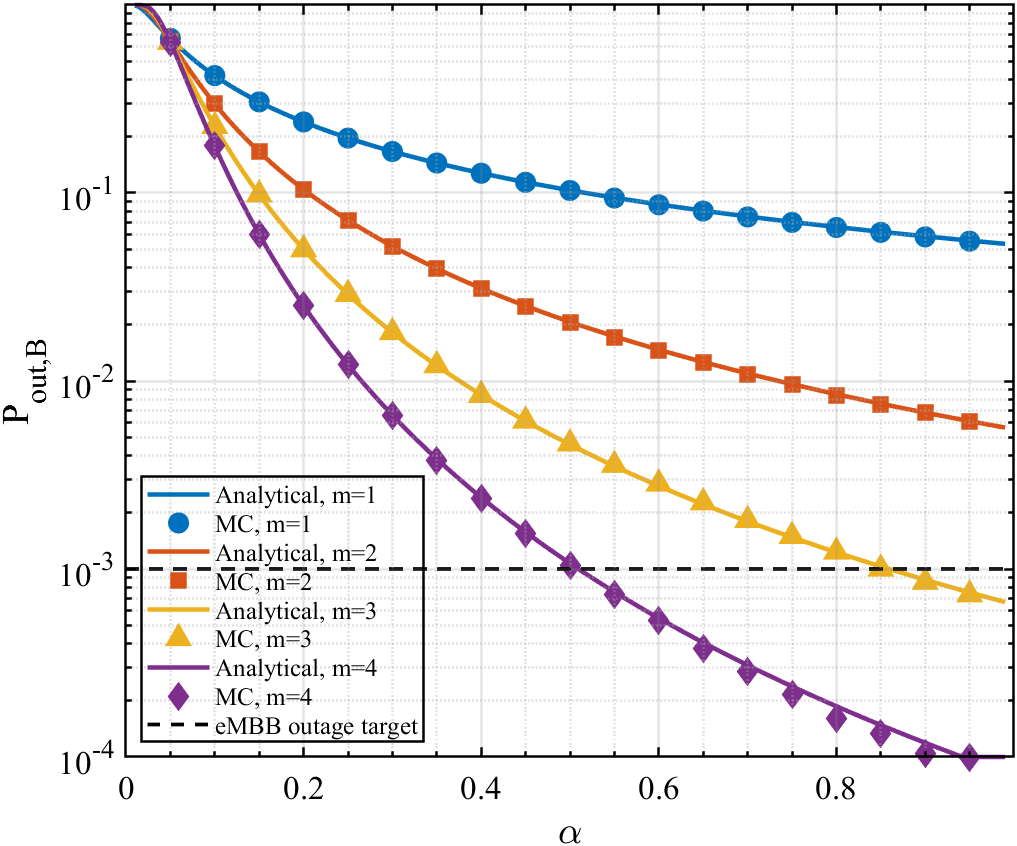
\includegraphics[width=\textwidth]{media/fig1_embb_outage.png}
        \caption{}
        \label{fig:sinr-left}
    \end{subfigure}\hfill
    \begin{subfigure}[b]{0.48\textwidth}
        \centering
        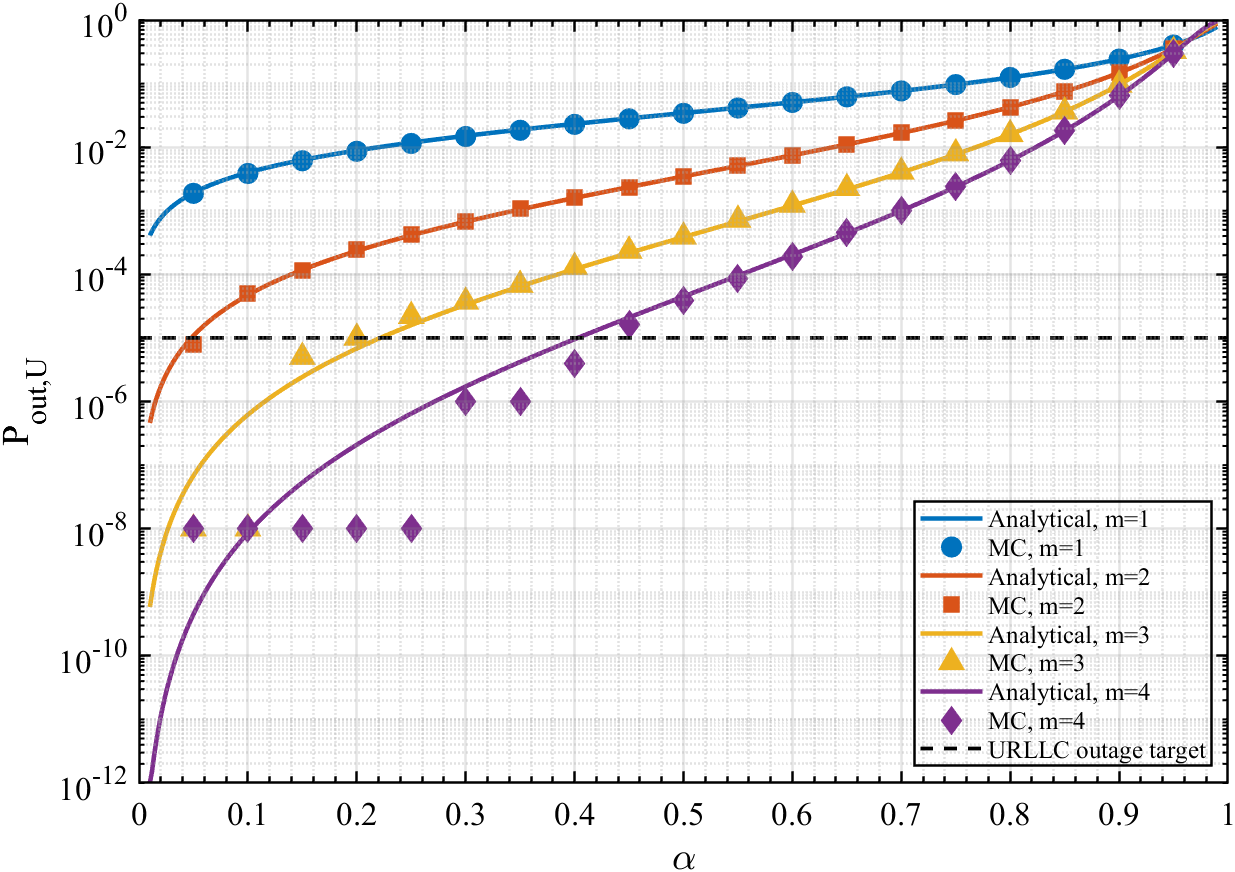
\includegraphics[width=\textwidth]{media/fig2_Urllc_outage.png}
        \caption{}
        \label{fig:capacity-right}
    \end{subfigure}
    \caption{\emph{Outage probability performance for eMBB and URLLC services versus power-allocation factor $\alpha$ across different Nakagami-$m$ fading parameters: (a) eMBB outage probability trends showing performance improvements as more power is allocated, and (b) URLLC outage probability behavior showing the impact of reduced power and increased residual interference during Successive Interference Cancellation (SIC) decoding.}}
    \label{fig:sinr-capacity-curves}
\end{figure}

\subsection{5.3 SINR and Capacity versus Alpha}\label{sinr-and-capacity-versus-alpha}

Figure 3 shows the capacity behavior associated with the allocated
multi-RB bandwidths. The eMBB mean-SNR approximation increases with
alpha, while the URLLC mean-SINR approximation decreases with alpha. The
eMBB capacity target is 50 Mbps and the URLLC capacity target is 1 Mbps.
Because eMBB has 14.4 MHz and URLLC has 3.6 MHz, the two services have
very different threshold requirements.

\begin{figure}[H]
    \centering
    \begin{subfigure}[b]{0.48\textwidth}
        \centering
        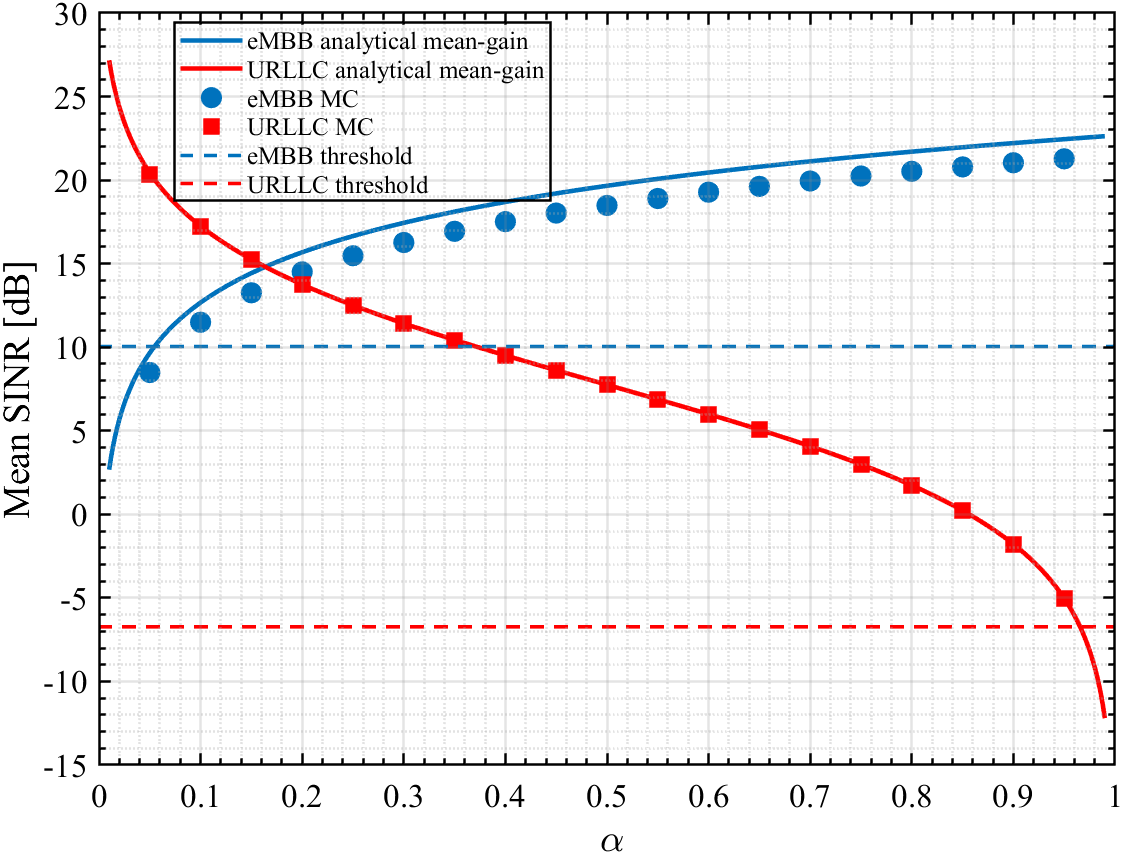
\includegraphics[width=\textwidth]{media/fig3_Mean_SINR.png}
        \caption{}
        \label{fig:sinr-left}
    \end{subfigure}\hfill
    \begin{subfigure}[b]{0.48\textwidth}
        \centering
        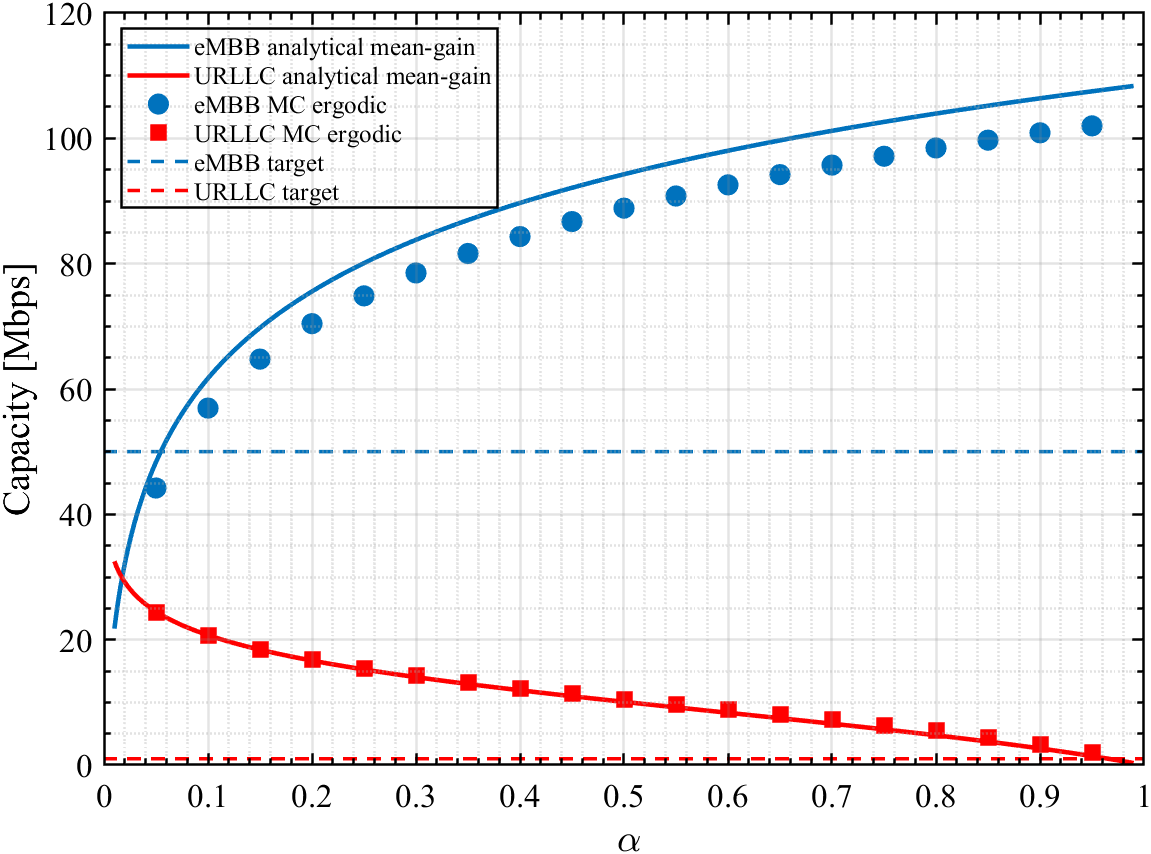
\includegraphics[width=\textwidth]{media/fig4_capacity.png}
        \caption{}
        \label{fig:capacity-right}
    \end{subfigure}
    \caption{\emph{Mean SINR and capacity performance comparison for eMBB and URLLC services as a function of the power-allocation factor $\alpha$: (a) Average SINR behavior demonstrating opposing trends for eMBB and URLLC as $\alpha$ varies, and (b) Achievable capacity relative to the 50 Mbps eMBB and 1 Mbps URLLC target thresholds over their respective 14.4 MHz and 3.6 MHz allocated bandwidths.}}
    \label{fig:sinr-capacity-curves}
\end{figure}

\subsection{5.4 Feasible Alpha and Optimal Alpha Results}\label{feasible-alpha-and-optimal-alpha-results}

The feasibility test uses all four constraints: eMBB outage, URLLC
outage, eMBB capacity, and URLLC capacity. At the baseline transmit
power of 30 dBm, the strict reliability requirements make the combined
feasible set empty for m = 1, 2, 3, and 4. This does not mean the model
failed; it means the selected QoS targets are too strict for the
baseline power and channel distances. The result is valuable because it
identifies when additional transmit power, improved channel conditions,
interference reduction, or relaxed reliability targets are required.

\begin{longtable}[]{@{}
  >{\raggedright\arraybackslash}p{(\linewidth - 8\tabcolsep) * \real{0.0896}}
  >{\raggedright\arraybackslash}p{(\linewidth - 8\tabcolsep) * \real{0.2420}}
  >{\raggedright\arraybackslash}p{(\linewidth - 8\tabcolsep) * \real{0.2621}}
  >{\raggedright\arraybackslash}p{(\linewidth - 8\tabcolsep) * \real{0.1979}}
  >{\raggedright\arraybackslash}p{(\linewidth - 8\tabcolsep) * \real{0.1979}}@{}}
\caption{Evaluation of individual and combined eMBB and URLLC QoS-feasible power-allocation factor $\alpha$ ranges at a baseline transmit power $P_t = 30\text{ dBm}$ under varying Nakagami-$m$ fading severities.}\tabularnewline
\toprule\noalign{}
\begin{minipage}[b]{\linewidth}\raggedright
m
\end{minipage} & \begin{minipage}[b]{\linewidth}\raggedright
eMBB \(α\) range satisfying
\(\mathbf{P}_{\mathbf{out,B}}\mathbf{\  \leq \ 10e - 3}\)
\end{minipage} & \begin{minipage}[b]{\linewidth}\raggedright
URLLC \(α\) range satisfying
\(\mathbf{P}_{\mathbf{out,U}}\mathbf{\  \leq \ 10e - 5}\)
\end{minipage} & \begin{minipage}[b]{\linewidth}\raggedright
Combined feasible \(α\) range
\end{minipage} & \begin{minipage}[b]{\linewidth}\raggedright
Decision
\end{minipage} \\
\midrule\noalign{}
\endfirsthead
\toprule\noalign{}
\begin{minipage}[b]{\linewidth}\raggedright
m
\end{minipage} & \begin{minipage}[b]{\linewidth}\raggedright
eMBB \(α\) range satisfying
\(\mathbf{P}_{\mathbf{out,B}}\mathbf{\  \leq \ 10e - 3}\)
\end{minipage} & \begin{minipage}[b]{\linewidth}\raggedright
URLLC \(α\) range satisfying
\(\mathbf{P}_{\mathbf{out,U}}\mathbf{\  \leq \ 10e - 5}\)
\end{minipage} & \begin{minipage}[b]{\linewidth}\raggedright
Combined feasible \(α\) range
\end{minipage} & \begin{minipage}[b]{\linewidth}\raggedright
Decision
\end{minipage} \\
\midrule\noalign{}
\endhead
\bottomrule\noalign{}
\endlastfoot
1 & None & None & None & Not feasible at 30 dBm \\
2 & None & 0.010 -- 0.048 & None & Not feasible at 30 dBm \\
3 & 0.860 -- 0.990 & 0.010 -- 0.222 & None & Not feasible at 30 dBm \\
4 & 0.510 -- 0.990 & 0.010 -- 0.403 & None & Not feasible at 30 dBm \\
\end{longtable}

To show how feasibility changes with transmit power, the simulation was
repeated over a range of \(P_{t}\) values. The minimum power values at
which a feasible \(α\) interval first appears are shown in Table 3.

\begin{longtable}[]{@{}
  >{\raggedright\arraybackslash}p{(\linewidth - 6\tabcolsep) * \real{0.1343}}
  >{\raggedright\arraybackslash}p{(\linewidth - 6\tabcolsep) * \real{0.2328}}
  >{\raggedright\arraybackslash}p{(\linewidth - 6\tabcolsep) * \real{0.2507}}
  >{\raggedright\arraybackslash}p{(\linewidth - 6\tabcolsep) * \real{0.3707}}@{}}
\caption{Impact of Nakagami-$m$ fading parameters on the power sensitivity and boundary limits of the QoS-feasible power-allocation factor $\alpha$ region for co-existing eMBB and URLLC services.}\tabularnewline
\toprule\noalign{}
\begin{minipage}[b]{\linewidth}\raggedright
m
\end{minipage} & \begin{minipage}[b]{\linewidth}\raggedright
Minimum \(\mathbf{P}_{\mathbf{t}}\) for feasible \(α\) region
\end{minipage} & \begin{minipage}[b]{\linewidth}\raggedright
First feasible \(α\) interval
\end{minipage} & \begin{minipage}[b]{\linewidth}\raggedright
Interpretation
\end{minipage} \\
\midrule\noalign{}
\endfirsthead
\toprule\noalign{}
\begin{minipage}[b]{\linewidth}\raggedright
m
\end{minipage} & \begin{minipage}[b]{\linewidth}\raggedright
Minimum \(\mathbf{P}_{\mathbf{t}}\) for feasible \(α\) region
\end{minipage} & \begin{minipage}[b]{\linewidth}\raggedright
First feasible \(α\) interval
\end{minipage} & \begin{minipage}[b]{\linewidth}\raggedright
Interpretation
\end{minipage} \\
\midrule\noalign{}
\endhead
\bottomrule\noalign{}
\endlastfoot
1 & No feasible region up to 60 dBm & None & Rayleigh fading is too
severe for the selected reliability targets. \\
2 & ≈ 47.0 dBm & 0.048 -- 0.049 & Feasibility appears only at very high
power and very narrow \(α\). \\
3 & ≈ 35.9 dBm & 0.221 -- 0.222 & Feasibility appears under moderate
improvement in fading/power. \\
4 & ≈ 31.1 dBm & 0.396 -- 0.403 & Feasibility appears close to the
baseline power because fading is less severe. \\
\end{longtable}

\begin{figure}[H]
    \centering
    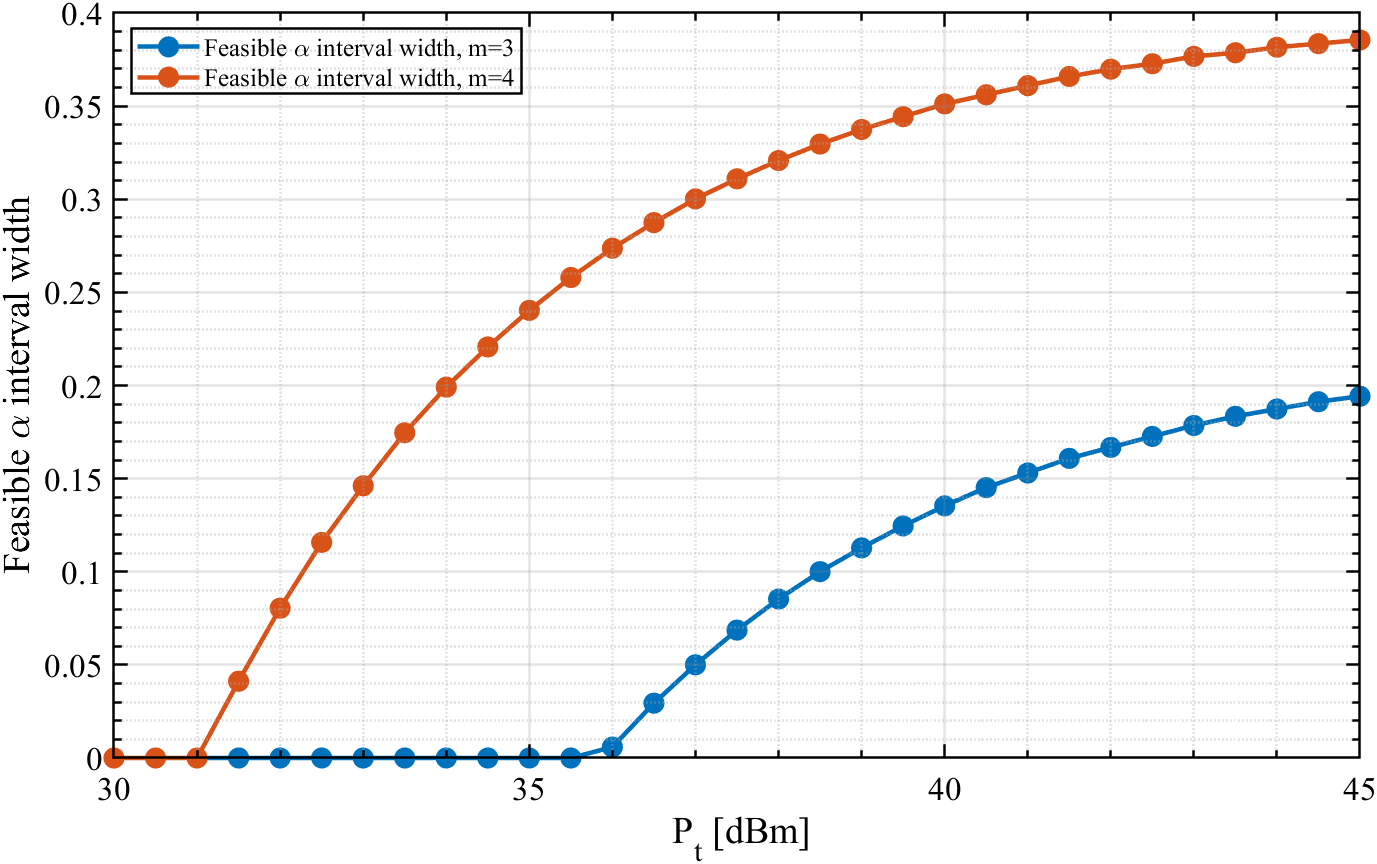
\includegraphics[height=5cm]{media/fig5_feasible_alpha_region.png}
    \caption{\emph{Width of the QoS-feasible power-allocation factor $\alpha$ region versus total transmit power $P_t$ for Nakagami fading parameters $m = 3$ and $m = 4$. The curves illustrate how less severe fading conditions expand the feasibility window and lower the minimum transmit power threshold required to simultaneously satisfy both eMBB and URLLC performance requirements.}}
    \label{fig:feasible-alpha-region}
\end{figure}

The optimal \(α*\) is meaningful only when the feasible set is non-empty.
For example, when m = 4 and \(P_{t}\) = 33 dBm, the feasible range is
approximately 0.255 \(≤ α ≤\) 0.403 and the throughput-maximizing feasible
value is \(α* ≈\) 0.403. This occurs because the total throughput is
dominated by the 50 Mbps eMBB target, so the optimizer selects the
largest feasible \(α\) before the URLLC outage constraint is violated.

\begin{longtable}[]{@{}
  >{\raggedright\arraybackslash}p{(\linewidth - 14\tabcolsep) * \real{0.1264}}
  >{\raggedright\arraybackslash}p{(\linewidth - 14\tabcolsep) * \real{0.0642}}
  >{\raggedright\arraybackslash}p{(\linewidth - 14\tabcolsep) * \real{0.1839}}
  >{\raggedright\arraybackslash}p{(\linewidth - 14\tabcolsep) * \real{0.0768}}
  >{\raggedright\arraybackslash}p{(\linewidth - 14\tabcolsep) * \real{0.1349}}
  >{\raggedright\arraybackslash}p{(\linewidth - 14\tabcolsep) * \real{0.1259}}
  >{\raggedright\arraybackslash}p{(\linewidth - 14\tabcolsep) * \real{0.1079}}
  >{\raggedright\arraybackslash}p{(\linewidth - 14\tabcolsep) * \real{0.1259}}@{}}
\caption{Throughput-maximizing optimal power-allocation factor $\alpha^*$ and the corresponding outage probability and capacity metrics for eMBB and URLLC services under non-empty QoS-feasible regions at selected transmit power $P_t$ and Nakagami-$m$ values.}\tabularnewline
\toprule\noalign{}
\begin{minipage}[b]{\linewidth}\raggedright
\[\mathbf{P}_{\mathbf{t}}\mathbf{\ (dBm)}\]
\end{minipage} & \begin{minipage}[b]{\linewidth}\raggedright
m
\end{minipage} & \begin{minipage}[b]{\linewidth}\raggedright
Feasible \(α\) range
\end{minipage} & \begin{minipage}[b]{\linewidth}\raggedright
\(α*\)
\end{minipage} & \begin{minipage}[b]{\linewidth}\raggedright
\(\mathbf{P}_{\mathbf{out,B}}\) at \(α*\)
\end{minipage} & \begin{minipage}[b]{\linewidth}\raggedright
\(\mathbf{P}_{\mathbf{out,B}}\) at \(α*\)
\end{minipage} & \begin{minipage}[b]{\linewidth}\raggedright
\(\mathbf{C}_{\mathbf{B}}\) at \(α*\) (Mbps)
\end{minipage} & \begin{minipage}[b]{\linewidth}\raggedright
\(\mathbf{C}_{\mathbf{U}}\) at \(α*\) (Mbps)
\end{minipage} \\
\midrule\noalign{}
\endfirsthead
\toprule\noalign{}
\begin{minipage}[b]{\linewidth}\raggedright
\[\mathbf{P}_{\mathbf{t}}\mathbf{\ (dBm)}\]
\end{minipage} & \begin{minipage}[b]{\linewidth}\raggedright
m
\end{minipage} & \begin{minipage}[b]{\linewidth}\raggedright
Feasible \(α\) range
\end{minipage} & \begin{minipage}[b]{\linewidth}\raggedright
\(α*\)
\end{minipage} & \begin{minipage}[b]{\linewidth}\raggedright
\(\mathbf{P}_{\mathbf{out,B}}\) at \(α*\)
\end{minipage} & \begin{minipage}[b]{\linewidth}\raggedright
\(\mathbf{P}_{\mathbf{out,B}}\) at \(α*\)
\end{minipage} & \begin{minipage}[b]{\linewidth}\raggedright
\(\mathbf{C}_{\mathbf{B}}\) at \(α*\) (Mbps)
\end{minipage} & \begin{minipage}[b]{\linewidth}\raggedright
\(\mathbf{C}_{\mathbf{U}}\) at \(α*\) (Mbps)
\end{minipage} \\
\midrule\noalign{}
\endhead
\bottomrule\noalign{}
\endlastfoot
33 & 4 & 0.255 -- 0.403 & 0.403 & 1.83e-04 & 9.99e-06 & 104.06 &
11.87 \\
36 & 3 & 0.216 -- 0.222 & 0.222 & 9.22e-04 & 1.00e-05 & 106.02 &
16.03 \\
36 & 4 & 0.128 -- 0.403 & 0.403 & 1.28e-05 & 9.99e-06 & 118.35 &
11.88 \\
39 & 3 & 0.108 -- 0.222 & 0.222 & 1.24e-04 & 9.98e-06 & 120.31 &
16.03 \\
39 & 4 & 0.064 -- 0.403 & 0.403 & 8.53e-07 & 9.99e-06 & 132.67 &
11.88 \\
\end{longtable}

\section{Chapter 6: Conclusion}\label{chapter-7-conclusion}

This project presented a QoS-aware resource allocation and performance
evaluation framework for 5G network slicing under Nakagami-m fading. The
study focused on the coexistence of eMBB and URLLC services, which
possess fundamentally different performance requirements. A practical
multi-resource-block uplink model was developed and implemented using
H-NOMA to enable simultaneous resource sharing between the two service
slices.

Analytical expressions for outage probability were derived under integer
Nakagami-m fading and used to evaluate the impact of resource allocation
decisions on system performance. The framework incorporated practical
bandwidth allocation, realistic noise modeling, distance-dependent path
loss, and QoS-constrained optimization of the power allocation factor \(α\).

The results demonstrated a clear trade-off between eMBB throughput and
URLLC reliability. Increasing the power allocated to eMBB improved
throughput and reduced eMBB outage probability but simultaneously
degraded URLLC reliability due to reduced transmit power and increased
interference during signal decoding. The study also showed that channel
fading conditions significantly influence the feasibility of resource
allocation decisions, with higher Nakagami-m values producing larger
QoS-feasible operating regions.

Furthermore, the analysis revealed that stringent QoS requirements can
lead to infeasible operating regions under limited transmit power,
emphasizing the importance of intelligent resource allocation mechanisms
in future wireless networks. Comparison with an H-OMA baseline
highlighted the benefits and limitations of non-orthogonal resource
sharing, demonstrating that H-NOMA provides greater flexibility for
balancing throughput and reliability when appropriate QoS-aware
allocation strategies are employed.

Overall, the proposed framework successfully identified and evaluated
resource allocation strategies capable of supporting heterogeneous 5G
service requirements under realistic fading environments. The findings
provide useful insights for the design of future network slicing and
radio resource management schemes in 5G and beyond wireless
communication systems.

Future work may extend the framework to multiple users per slice,
dynamic traffic conditions, adaptive scheduling algorithms,
machine-learning-based resource allocation techniques, imperfect SIC
scenarios, and emerging 6G network architectures.

% ... this is the end of your last paragraph of text.

\clearpage

\printbibliography[title={References}]
\addcontentsline{toc}{section}{References}

\end{document}
